\chapter{Laser Pieces}
%the sum of the whole is greater than the parts 

The laser system consists of several components arranged together on a breadboard. 

\begin{figure}
    \centerline{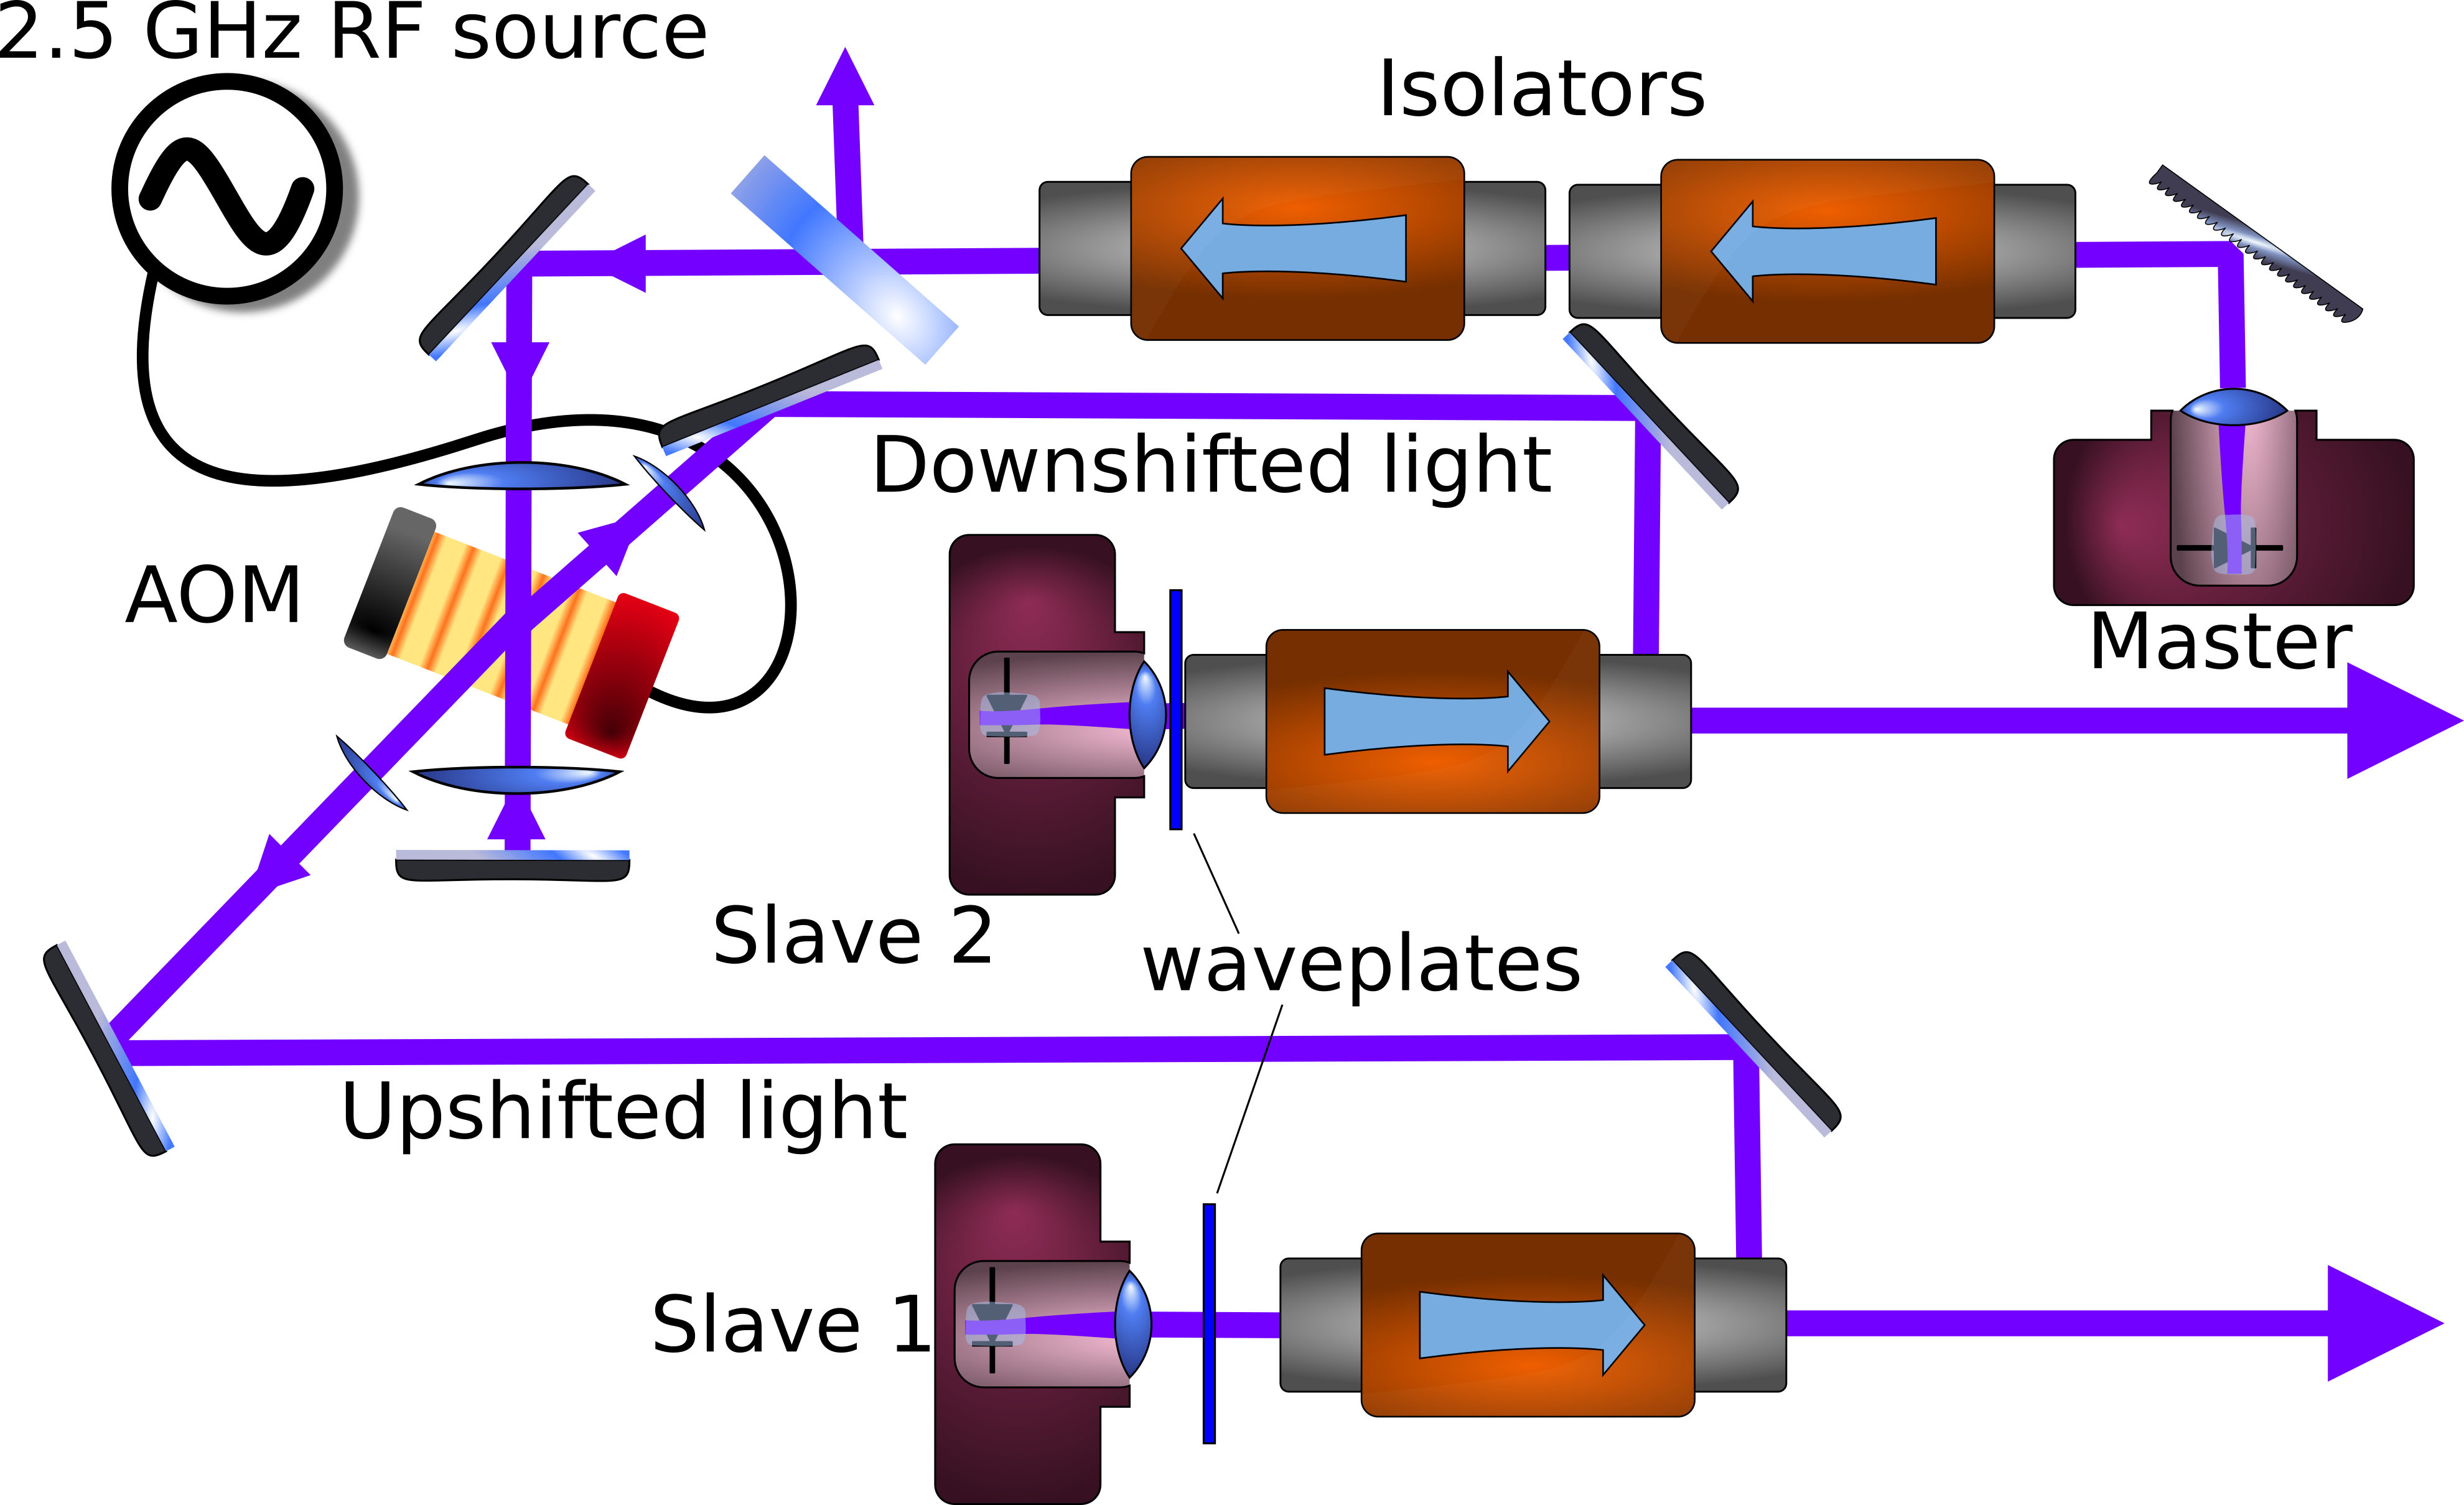
\includegraphics[width=1\textwidth]{diagramOfSetup3}}
    \caption[Numerical method]{\label{fig:diagramOfSetup}
    Just plot the magnitude of the vertically polarized component as a function of $\theta_1$. I used the slider to control $\theta_2$. Obviously, I'll illustrate this better at some point.}
\end{figure}


There are three separate laser diodes in housings. One of them is designated the "Master" laser. The master laser is grating stabilized using an extended cavity formed by a  %look this up
lines/mm diffraction grating mounted on a piezoelectric mount.  

The master laser passes through two optical isolators. It is then passed through a pair of waveplates and a polarizing beam cube, which serves the dual purpose of allowing us to attenuate the portion of the beam that goes through the AOM and splitting off a beam that can be used in our spectrum analyzer. 

After this, the laser is passed twice through an Acousto-optic Modulator (AOM). This splits off two beams, one of which is shifted upwards by 2.5 GHz and the other of which is shifted downward by 2.5 GHz. These two beams are then coupled through optical isolators into the two slave lasers. The outputs of these two lasers are what we use in our experiment to achieve stimulated Raman transitions. 


